A string is a sequence of symbols/characters/letters (all equivalent), symbols are drawn from an alphabet $\Sigma$ and we state that $\sigma = |\Sigma|$.
Moreover in the sorting problem we have: $S[1, n]$ as our sequence of strings , $N$ as the total length of all the strings, $n$ as the number of strings and $L = \frac{N}{n}$ as the average length of the strings.

Strings are stored in memory in this way:
\begin{figure}[H]
    \centering
    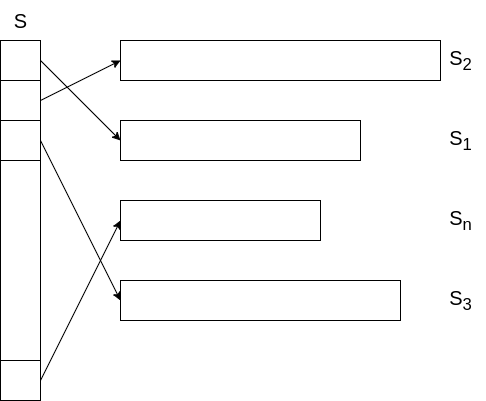
\includegraphics[width=225px]{images/5_String_sorting/string_storage.png}
\end{figure}
we could use the already analyzed \verb|qsort| procedure:
\begin{verbatim}
    qsort(array, #items, size_of_obj, cmp_function)
\end{verbatim}
in which we sort the pointers which points to the string and the comparison function analyzes the strings.

Qsort is a comparison based algorithm which executes $O(nlog_2 n)$ comparisons, since we are dealing with strings each comparison is $O(L)$ so the total cost of sorting using qsort is $O(L \cdot n \cdot log_2 n) = O(N \cdot log_2 n)$.

In I/O model tough we have some drawbacks: since in quick-sort when $[l,r]$ is small enough we apply insertion sort to exploit cache, we lose every boost because strings are stored away from the pointer array, so no improvement.

\section{Lower bound}
We can prove a lower bound for string sorting:
\begin{itemize}
    \item we must sort the first character of each string to begin with, so $\Omega(n \cdot log_2 n)$;
    \item let's suppose to have:
    \begin{itemize}
        \item $S_1 = $abaco;
        \item $S_2 = $abate;
        \item $S_3 = $abb.
    \end{itemize}
    we can estimate the number of characters we need to scan to lexicographically sort those strings:
    \begin{itemize}
        \item for $S_1$: $d_1 = 4$;
        \item for $S_2$: $d_2 = 4$;
        \item for $S_3$: $d_3 = 3$.
    \end{itemize}
    we call those numbers \emph{distinguishing prefix}, moreover we define $d = \sum_s d_s$ as the totality of those prefixes.
    In the end for this part we have $\Omega(d)$.
\end{itemize}
So a theoretical lower bound for this problem is:
$$
    \Omega( n \cdot log_2 n + d)
$$
in terms of time/comparison.

It's a bit like having strings like:
\begin{figure}[H]
    \centering
    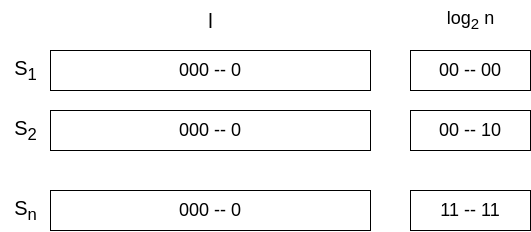
\includegraphics[width=250px]{images/5_String_sorting/string_sorting_lower_bound.png}
\end{figure}
for each of those strings we have $d_i = l + log_2 n$, so $d = \sum_s (l + log_2 n) = l \cdot n + n \cdot log_2 n$, so qsort would take $O(L \cdot n \cdot log_2 n)$ since $L$ is the average in our case we have:
$$
    O((l + log_2 n) \cdot n \cdot log_2 n) = O(l \cdot n \cdot log_2 n + n \cdot log_2^2 n)
$$, we have the term $log_2^2 n$ more than the lower bound, so qsort is at least a $log_n$ factor from the optimal.

\section{Radix Sort}
We have two different approaches:
\begin{itemize}
    \item Most Significant Digit first (MSD): in which we scan strings left to right;
    \item Least Significant Digit first (LSD): in which we scan strings right to left
\end{itemize}

\subsection{MSD}
Let's start with an example:
$$
    S = \{007, 017, 042, 911, 991\}
$$
we have $\sigma = 10$, $\Sigma = \{0, 1, \_, 9\}$, $n = 5$, $N = 15$.
We start with an array of size $\sigma$, we scan each item and place it inside the right bucket according to the first character of each element:
\begin{figure}[H]
    \centering
    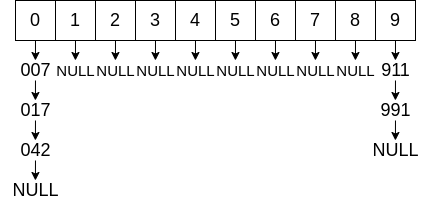
\includegraphics[width=250px]{images/5_String_sorting/radix_sort_MSD_0.png}
\end{figure}
then for each bucket we create a new array of size $\sigma$ and repeat the process for each element in that bucket:
\begin{figure}[H]
    \centering
    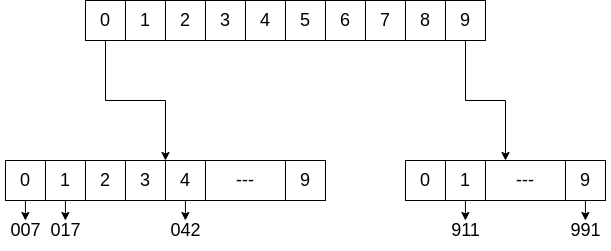
\includegraphics[width=275px]{images/5_String_sorting/radix_sort_MSD_1.png}
\end{figure}
now we have just one string in each bucket, so scanning the leaves of this tree from left to right we have our strings sorted.
Of course we don't finish at the same level for each bucket but we always build a tree-like structure.

An upper bound for the arrays we need to create can be: for each string we have we need to create at most $d_s$ nodes, of course a lot of them are common between strings but we can state that:
$$
    \#nodes \leq d = \sum_s d_s
$$
So total space complexity is $O(d \cdot \sigma)$, and since the building of the tree is the sorting itself the sorting time is the same as the space complexity, so $O(d \cdot \sigma)$.

Since the alphabet is constant we drop it from the big $O$ notation, so in the end our time complexity for sorting is $O(d)$ which is lower than the upper bound we proved before.
That's because the Radix sort is not a comparison-based algorithm and the lower bound we stated before is only applicable to those kind of algorithms!

\subsubsection{Trie data structure}
The tree we have built during radix sort is a particular data structure called \emph{trie}.
It is a tree in which each node has $\sigma$ pointers to nodes, basically it's a $\sigma$-ary tree.

It's a data structure a lot efficient for searching operations but it's inefficient in space, which is $O(d \cdot \sigma)$, and if the alphabet is huge we have a lot of space, most of the time wasted for null pointers.

It is efficient in search operation because we traverse the tree, with the known key in $O(p)$ with $p = \#$length of the string we are looking for.

To avoid wasting space in null pointers in the case of big alphabets we can use an hash-table or a BST to store the tuples: $<character, ptr>$.

Using the hash-table approach we need to add an hash-table on each node whose size is proportional to number of pairs stored in that node (which is the number of edges outgoing from that node).
Using an hash-table we could potentially have collisions but since size is proportional to keys access is still in $O(1)$ on average.

Using the BST we have access in $O(log_2 \sigma)$ because we have at most $\sigma$ nodes in BST, if it is balanced, of course.

Of course using one of the methods above lead us to lose the order between outgoing edges so if we want to use MSD Radix sort the algorithm becomes:
\begin{itemize}
    \item build the trie in: $\sum_s O(1) \cdot d_s = O(d)$ on average;
    \item sort each hash table and traverse the edges in order, using qsort we'll have $O(\#edges \cdot log_2 \#edges)$ let's call $e_u$ the average number of edges for each node: $O(e_u \cdot log_2 e_u)$.
\end{itemize}
so in the end:
$$
    \sum_u O(e_u \cdot log_2 e_u) = O\left(\sum_u e_u \cdot log_2 e_u\right)
$$
we can upper bound $e_u \leq \sigma \forall u$:
$$
    O\left(\sum_u e_u \cdot log_2 e_u\right) \leq O\left(\sum_u e_u \cdot log_2 \sigma\right) = O\left(log_2 \sigma \cdot \sum_u e_u\right) 
$$
and we have the sum of all the edges which is equal to the number of nodes, so we can upper bound it too:
$$
    O\left(log_2 \sigma \cdot \sum_u e_u\right) \leq O(d \cdot log_2 \sigma)
$$

So this algorithm takes $O(d \cdot log_2 \sigma)$ time and $O(d)$ space.

\subsection{LSD}
Given the sequence $S=\{ 017, 042, 665, 111, 007 \}$ we scan the sequences backwards, exploiting a stable sort to sort the sequences by the first digit. Since we use a stable sort the elements with the same digit will keep the relative order among them.
As stable sort we use counting sort which runs in $O(\# keys + |\Sigma|)$.

\begin{table}[H]
    \centering
    \begin{tabular}{c c c c}
        starting & $i=3$ & $i=2$ & $i=1$  \\
        017 & 111 & 007 & 007 \\
        042 & 042 & 111 & 017 \\
        665 & 665 & 017 & 042 \\
        111 & 017 & 042 & 111 \\
        007 & 007 & 665 & 665 \\
    \end{tabular}
    \caption{LSD sorting in action}
\end{table}
as we can see in the example above the strings are sorted at the end of the last step.

\subsubsection{Complexity}
The total complexity is $\#digits \cdot O(\text{stable sort})$ so:
$$
    O(L \cdot (n + \sigma)) = O(n \cdot L + \sigma \cdot L) = O(N + \sigma \cdot L) = O(N)
$$
so we have $O(N)$ time and $O(N)$ space.

\subsubsection{Proof of correctness}
A simple proof of correctness can be: let's start from two strings $x$ and $y$, and we pose the hypothesis that $x < y$, we want to prove that if $x < y$ then the LSD radix sort will sort them according to that statement.
We build those strings as generic:
\begin{figure}[H]
    \centering
    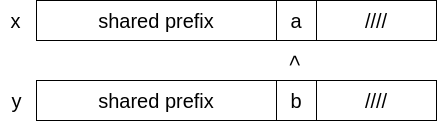
\includegraphics[width=250px]{images/5_String_sorting/LSD_proof.png}
\end{figure}
since we scan from right to left we don't care of the content of the tail of those strings, once we get to $a$ and $b$ we sort them with $x$ before $y$, then for all the characters in the shared prefix we use a stable sort so the relative order between $x$ and $y$ remains the same until the end.

Since it's true for each pair of strings it is true for all sets of strings.

\subsubsection{A better complexity proof}
Let's assume we have binary strings, so strings composed just with ones and zeroes: instead of comparing them bit by bit we group them by $r$ bits, so we have $\frac{b}{r}$ groups each of $r$ bits.
Now we have $\sigma = 2^r$.

Applying counting sort over there will give us $\frac{b}{r}$ phases, each costing $n + 2^r$ so $O\left( \frac{b}{r}(n+2^r) \right)$ which has minimum for $r = log_2 n$:
$$
    O\left( \frac{b}{log_2 n} \cdot (n + 2^{log_2 n}) \right) = O\left( \frac{b}{log_2 n} (n+n) \right) = O\left( \frac{n \cdot b}{log_2 n} \right) = O\left( \frac{N}{log_2 n} \right)
$$
So the actual complexity is $O\left( \frac{N}{log_2 n} \right)$.

So the original lower bound was $\Omega(n \cdot log_2 n + d)$ but we have a better lower bound of $O\left( \frac{N}{log_2 n} \right)$ because we aren't using comparison based approach.

NB: this algorithm is bad in case of short distinguish prefix, in that case MSD is better because those prefix are found faster!

\subsection{Multi-key Quicksort}
The algorithm is:
\begin{verbatim}
    MKQ(R, i)
        if (|R| <= 1)
            return R
        else
            choose a pivot string p in R
            R_less = {s in R : s[i] < p[i]}
            R_equals = {s in R : s[i] = p[i]}
            R_greater = {s in R : s[i] > p[i]}

            A = MKQ(R_less, i)
            B = MKQ(R_equals, i+1)
            C = MKQ(R_greater, i)

            return A | B | C
\end{verbatim}

We have an invariant for this algorithm: all the strings in the set $R$ share $i-1$ characters, so in terms of $i-1$ characters, they are the same string.
Then we concentrate on $i$-th characters: we put the strings in $R_<$, $R_=$, $R_>$ according to the lexicographical order of that character, in the end we partitioned those strings by that character that could be the last of the distinguish prefix.
That's a verbose correctness proof.

Of course we invoke the procedure as \verb|MKQ(S, 1)|.

\subsubsection{Complexity}
For sure we can say that:
\begin{itemize}
    \item $|R_<|, |R_>| < |R|$: because at least $p$ won't be inside one of them so the size of those sets will shrink;

    \item $|R_=| \leq |R|$: they are equals when all characters are the same one. That case is bad with recursion but on the next iteration we will go to the next index and since we recurse until $i \leq max_i |s_i|$, so it will terminate eventually.
\end{itemize}
Let's define $n = \#$strings and $N = $total length of all strings.
As we said when picking $s \in R$ we have two cases:
\begin{itemize}
    \item $s[i] < p[i]$ and so $s \in R_<$ and $s[i] > p[i]$ and so $s \in R_>$;
    \item $s[i] = p[i]$ and $s \in R_=$ but we increment $i$ so after some recursion level we will fall in the first case.
\end{itemize}
first case is the same as quick-sort so we could even end up in linear number of recursions, in the worst case but for our analysis we will state that on average we will pick a random pivot such that we'll have:
$$
    |R_<| \approx |R_>| \approx \frac{|R|}{2}
$$
so we will have $O(log_2 |S|)$ recursive steps on average.

For the string $s$ the number of recursive call is $O(log_2n + d_s)$, in total we have:
$$
    \sum_s O(log_2 n + d_s) = O\left( \sum_s log_2 n + d_s \right) = O(n \cdot log_2 n + d)
$$
so on average we meet the lower bound.

\subsubsection{Ternary search tree}
Starting from Multi-key quick-sort we can build a ternary search tree (or ternary trie) which has the following structure:
\begin{figure}[H]
    \centering
    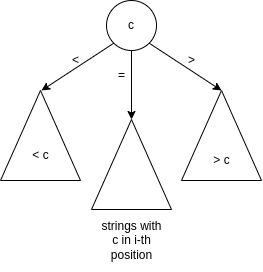
\includegraphics[width=175px]{images/5_String_sorting/ternary_search_tree.png}
\end{figure}
Each node has 3 pointers, going to the left and right arms we don't advance the position, we do it going in the middle element.

Example: insert the elements from the set $S = \{ cat, abi, cast \}$:
\begin{figure}[H]
    \centering
    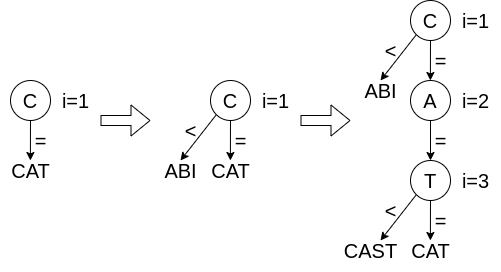
\includegraphics[width=300px]{images/5_String_sorting/TST_example_1.png}
\end{figure}
in the third insertion we insert first the node $A$ because \emph{cat} and \emph{cast} share the prefix \emph{ca}, then we choose one of those strings (in this instance \emph{cat}) and we store it in the third node, then we need to store \emph{cast}, since $s < t$ we put that string on the left arm.

Of course TST could be unbalanced but if strings are inserted randomly we have that a string $s$ gets a path of length: $O(|d_s| + log_2 n)$.
Then each node needs only an array of 3 pointers and one splitting character.
